%  -*- TeX-master:  "main"; fill-column: 72 -*-

\section{Proposed syntax and semantics}
\label{syntax}

In this section, we define the syntax and semantics of the Arrays package for SBML Level~3 Version~1.   We describe the various data types and constructs defined in this package, then in \sect{examples}, we provide complete examples of using the constructs in example SBML models.

%  -----------------------------------------------------------------------------
\subsection{Namespace URI and other declarations necessary for using this package}
\label{xml-namespace}

Every SBML Level~3 package is identified uniquely by an XML namespace URI.
For an SBML document to be able to use a given SBML Level~3 package, it
must declare the use of that package by referencing its URI.   The following
is the namespace URI for this version of the Arrays
package for SBML Level~3 Version~1:
\begin{center}
\uri{http://www.sbml.org/sbml/level3/version1/arrays/version1}
\end{center}

In addition, SBML documents using a given package must indicate whether
understanding the package is required for complete mathematical
interpretation of a model, or whether the package is optional.   This is
done using the attribute \token{required} on the \token{<sbml>} element in
the SBML document.   For the Arrays package, the value of
this attribute must be set to \val{true}.
The following fragment illustrates the beginning of a typical SBML model
using SBML Level~3 Version~1 and this version of the Arrays package:

\begin{example}
<?xml version="1.0" encoding="UTF-8"?>
<sbml xmlns="http://www.sbml.org/sbml/level3/version1/core" level="3" version="1"
  xmlns:arrays="http://www.sbml.org/sbml/level3/version1/arrays/version1" arrays:required="true">
\end{example}

\subsection{Primitive data types}

Section~3.1 of the \sbmlthreecore specification defines a number of primitive data types and also uses a number of XML Schema 1.0 data types~\citep{biron:2000}.   More specifically, we make use of \primtype{SId},  \primtype{string},  \primtype{int}, and \primtype{SIdRef}.

% The Arrays package also defines two new primitive data types defined below.

%% QUESTION: IS THIS STILL NEEDED?   PERHAPS NOT FOR L3V2.

%  \subsubsection{\emph{Type}  \primtype{DimSId}}

% The type \primtype{DimSId} is derived from \primtype{SId}  (SBML Level 3 Version 1 Core specification Section 3.1.7) and has identical syntax. The \primtype{DimSId} type is used as the data type for the identifiers of \Dimension objects. The purpose of having a separate type for such identifiers is to enable the space of possible dimension identifier values to be separated from the space of all other identifier values in SBML.   The scope of the \primtype{DimSId} is local to the enclosing object definition and is not visible outside the object definition.   The equality of \primtype{DimSId} values is determined by an exact character sequence match; i.e., comparisons of these identifiers must be performed in a case-sensitive manner.

%\subsubsection{\emph{Type}  \{ 0, 1 \}}

%This type is simply the \primtype{int} type limited to the values of 0 and 1.

\subsection{Dimensions}
\label{sec:dimension}

As shown in \ref{fig:dimensions_uml}, the arrays package extends the \SBase class from core SBML with the addition of a list of \Dimension objects.   An object with a list of dimensions is an array, and the number of dimensions is equivalent to the number of \Dimension objects in the list.   %%Currently, SBML objects are restricted to at most three dimensions.

\begin{figure}[ht]
    \centering
    % Requires \usepackage{graphicx}
    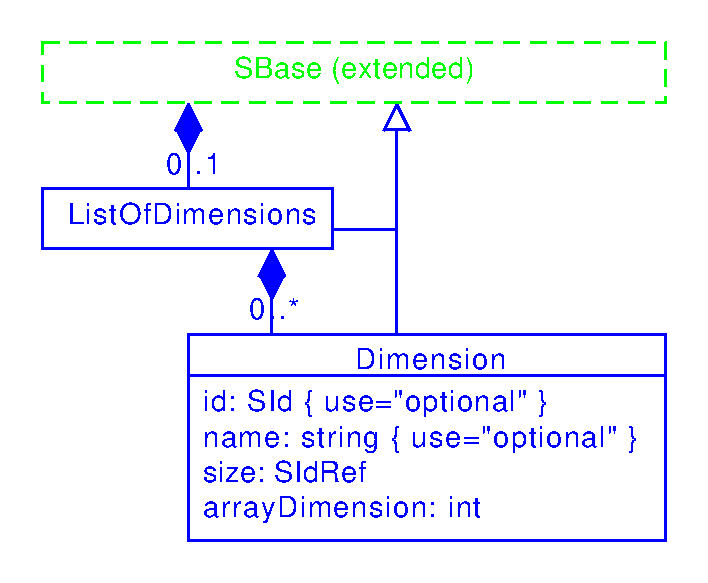
\includegraphics{images/dimensionsUML.pdf}
    \caption{A UML representation of the extended \SBase, \ListOfDimensions, and \Dimension classes. See \ref{conventions}} for conventions related to this figure.
    \label{fig:dimensions_uml}
\end{figure}

%\subsubsection{Dimension}

\paragraph{The \primtype{id} attribute}

The \Dimension object has an optional attribute, \primtype{id}, used to give the dimension an identifier.   The value of \primtype{id} must conform to the syntax permitted by the \primtype{SId} data type described in Section 3.1.7 of the SBML Level 3 Version 1 Core specification.   The scope of the \primtype{id} attribute is local to the enclosing object definition and is not visible outside the object definition.  \changed{It may therefore be used in mathematical expressions within the enclosing object definition, but only by reference--it may not be assigned a value by a \Rule or other assignment.  When used, it is similar to the \token{time} variable from SBML core, or the \CoordinateComponent element from the Spatial specification: it represents a 'domain' over which the model is defined.  In context, then, it represents the set of all integers from 0 to the \Dimension's \token{size}.}

\changed{The value of the \token{id} attribute must be unique among the \primtype{SId} values both local to the object and global to the \Model.  This means that if a \Parameter in the same \Model has an \token{id} of \val{a0}, and the same parent object has another \Dimension with an \token{id} of \val{b0}, this \Dimension must not have a value of either \val{a0} or \val{b0}.  Similarly, if a parent \Reaction of a \Dimension has a \LocalParameter child of its \KineticLaw with an id of \val{c0}, that \Dimension may not be given an \token{id} of \val{c0}.  However, two different \AssignmentRule elements in the same \Model may each be given a \Dimension with an \token{id} of \val{d0}, without semantic overlap.  In general,} the \primtype{id} attribute must be used as described in Section 3.3 of the SBML Level 3 Version 1 Core specification.


\paragraph{The \primtype{name} attribute}

\Dimension also has an optional \primtype{name} attribute, of type \primtype{string}  (see Section 3.1.1 and Section 3.3 of the SBML Level 3 Version 1 Core specification).

\paragraph{The \primtype{size} attribute}

Each dimension of an array has a fixed size which is set with the \primtype{size} attribute.   The size attribute is of type \primtype{SIdRef}  (see Section 3.1.8 of the SBML Level 3 Version 1 Core specification) and must refer to a \Parameter object instance defined in the model.   The \Parameter referenced must be \primtype{constant}, scalar \changed{(that is, it may not itself have a \Dimension child)}, and have a defined initial value \changed{that must be a positive non-zero integer}.

{\color{red} Lucian: \notice Check to see if 'non-zero' is a requirement.  It also might still be worth having a discussion about the 'defined initial value'.}


\paragraph{The \primtype{arrayDimension} attribute}

The \primtype{arrayDimension} attribute specifies which dimension is defined by this \Dimension object.
%Currently, the only allowed values for \primtype{arrayDimension} are 0,
%1, and 2 (i.e., at most 3-dimensional arrays).   Also,
The only allowed values for \primtype{arrayDimension} are non-negative integer values (e.g. $0,1,2,\dots,n$).   Also, there can be at most one \Dimension for each possible value of \primtype{arrayDimension}.
%Finally, if a list of dimensions includes a
%\Dimension with \primtype{arrayDimension} value of 1, it must also
%include one with value 0.   Similarly, if it includes a \Dimension with
%\primtype{arrayDimension} value of 2, it must include ones with value 0
%and 1, as well.  This rule applies for higher dimensions.
Finally, if a list of dimensions includes a \Dimension with \primtype{arrayDimension} value of $n$, it must also
include \Dimension objects with value $n-1, n-2, \dots , 1, 0$.

\paragraph{Example}

As an example, a $10 \times 10$ array of compartments \changed{\val{Cell}} could be defined as:

\begin{example}
<listOfCompartments>
    <compartment id="Cell" constant="true" spatialDimensions="3" size="1">
        <arrays:listOfDimensions
            xmlns:arrays="http://www.sbml.org/sbml/level3/version1/arrays/version1">
            <arrays:dimension arrays:id="d0" arrays:size="n" arrays:arrayDimension="0"/>
            <arrays:dimension arrays:id="d1" arrays:size="n" arrays:arrayDimension="1"/>
        </arrays:listOfDimensions>
    </compartment>
</listOfCompartments>
<listOfParameters>
    <parameter id="n" constant="true" value="10"/>
</listOfParameters>
\end{example}

\paragraph{Dimension usage}
\label{sec:dimensionUsage}

In SBML Level~3 Core, the following objects are permitted to have a \ListOfDimensions:

\nolinenumbers
\begin{multicols}{3}
\begin{itemize}\setlength{\parskip}{-0.2ex}
\item \Compartment,
\item \Constraint,
\item \Event,
\item \EventAssignment,
\item \InitialAssignment,
\item \Parameter,
\item \Reaction,
\item \Rule,
\item \Species, and
\item \SpeciesReference.
\end{itemize}
\end{multicols}
\linenumbers

All other SBML Level~3 Core objects are not permitted to have a \ListOfDimensions:

\nolinenumbers
\begin{multicols}{3}
\begin{itemize}\setlength{\parskip}{-0.2ex}
\item \Delay,
\item \FunctionDefinition,
\item \KineticLaw,
\begin{blockChanged}
\item \ListOfUnits,
\item \ListOfUnitDefinitions,
\item \ListOfLocalParameters,
\item \ListOfCompartments,
\item \ListOfSpecies,
\item \ListOfParameters,
\item \ListOfInitialAssignments,
\item \ListOfRules,
\item \ListOfConstraints,
\item \ListOfReactions,
\item \ListOfSpeciesReferences,
\item \ListOfEvents,
\item \ListOfEventAssignments,
\end{blockChanged}
\item \LocalParameter,
\item \Model,
\item \Priority,
\item \Trigger,
\item \Unit, and
\item \UnitDefinition.
\end{itemize}
\end{multicols}
\linenumbers

All SBML objects defined by packages that inherit from \SBase are permitted to have a \ListOfDimensions unless it is explicitly disallowed in the corresponding package specification, \changed{with the exception of any \ListOf class.  None of these arrays package classes (\Dimension, \Index, \ListOfDimensions, and \ListOfIndices)} are permitted to have a \ListOfDimensions.

It is important to note that it is assumed that all elements of arrays created in this way share the same attribute values.   For example, \changed{if a \Species is set \token{boundaryCondition}=\val{true}, all \Species in the array are then defined as boundary species.  Similarly, every element in the array will have the same \token{units}.}  \changed{If a \token{size} is specified for a \Compartment, or a \token{value} for a \Parameter,} then every element of the array takes that initial value.   To specify different initial values to different elements of an array, an \InitialAssignment can be used, \changed{but generally, there is no way to alter the values of individual attributes of elements in an array.}

\subsection{Indices}
\label{sec:index}

As shown in \ref{fig:indices_uml}, the arrays package extends the \SBase class from core SBML with the addition of a list of indices.
%Each index in this list is used to specify an array index for a reference to an arrayed object specified in an attribute for this SBML element.
Each index in this list is used to specify an array index. The array index is used to reference an arrayed object specified in an attribute for this SBML element.
Each arrayed object specified in an attribute can have at most one index for each dimension specified for that object.
%For example, if the referenced object is a one-dimensional array, it
%can have one index.   If the referenced object is a two-dimensional
%array, it can have two indices.   In these cases, the referenced object
%is a scalar.   Note that if a two-dimensional array has only one index,
%the reference would return a one-dimensional array specified by this index.   If no index is specified, then the entire array is being referenced.
% Note that \SBase objects containing \token{SIdRef}  objects with a \ListOfDimensions that the
%   object refencing the arrayed object is required to have  a \ListOfIndices in which the number of
%   \Index objects is required match the number of dimensions of the referenced arrayed object. For example, assume there is an \AssignmentRule R that is assigning a value to \Parameter P. Furthermore, assume that P is a two-dimensional array.  Then, it must be the case that R has two \Index objects to reference a single value of P.

Note that \SBase objects containing \token{SIdRef}  objects with a
\ListOfDimensions are required to have  a \ListOfIndices, where the number of
  \Index objects for each particular object you are indexing is required
  to match the number of dimensions of the referenced arrayed
  object. For example, assume there is an \AssignmentRule that is
  assigning a value to \Parameter. Furthermore, assume that
  the \Parameter is a two-dimensional array.  Then, it must be the case
  that the \Rule has two \Index objects to reference a single value of
  the \Parameter.
\begin{figure}[ht]
    \centering
    % Requires \usepackage{graphicx}
    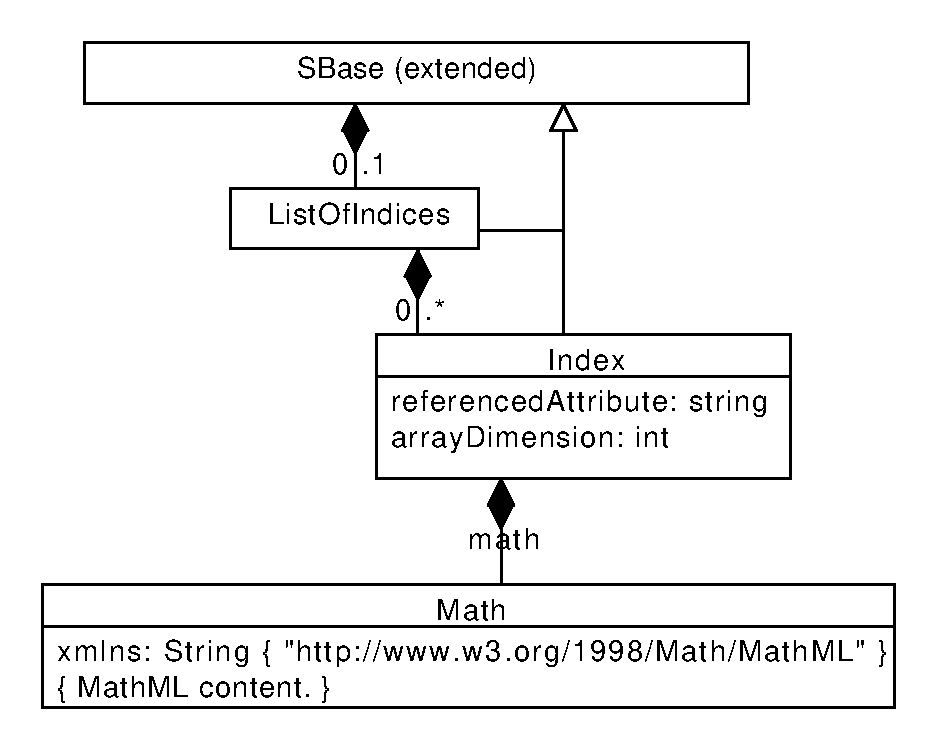
\includegraphics{images/indicesUML.pdf}
    \caption{A UML representation of the extended \SBase, \ListOfIndices, and \Index classes. See \ref{conventions}} for conventions related to this figure.
    \label{fig:indices_uml}
\end{figure}

\paragraph{The \primtype{referencedAttribute} attribute}

The \primtype{referencedAttribute} attribute specifies the attribute of the SBML object to which this index is referencing.

\paragraph{The \primtype{arrayDimension} attribute}

The \primtype{arrayDimension} attribute specifies which dimension this index corresponds to.
%Currently, the only allowed values for \primtype{arrayDimension} are 0,
%1, and 2 (i.e., at most 3-dimensional arrays can be indexed).
%Also, there can be at most one \Index for each possible value of
%\primtype{arrayDimension}.   Finally, if a list of indices includes an
%\Index with \primtype{arrayDimension} value of 1, it must also include
%one with value 0.   Similarly, if it includes an \Index with
%\primtype{arrayDimension} value of 2, it must include ones with value 0
%and 1, as well.
The only allowed values for \primtype{arrayDimension} are
  non-negative integer values. Also, there can be at most one \Index for
  each possible pair of values
\primtype{arrayDimension} and \primtype{referencedAttribute}. Finally, if a list of indices includes a
\Index with \primtype{arrayDimension} value of $n$, it must also
include \Index objects with value $n-1, n-2, \dots , 1, 0$ for each \primtype{referencedAttribute} attribute.

\paragraph{The \primtype{math} element}

The \primtype{math} element provides a mathematical expression which is evaluated to determine the index value for the reference.   Note that arrays are 0-based which means that an object of size $n$ can have index values between 0 and $n-1$.   When an index value computes to a value outside this range during \changed{a simulation or analysis}, this is an \emph{array out-of-bounds} error and \changed{the program} should terminate and report this error to the user.

\paragraph{Example}

The example below copies a reverse copy of the array in parameter x into parameter y.

\begin{example}[showstringspaces=false]
<listOfParameters>
  <parameter id="n" constant="true" value="10"/>
  <parameter id="X" constant="false" value="0">
    <arrays:listOfDimensions xmlns:arrays="http://www.sbml.org/sbml/level3/version1/arrays/version1">
      <arrays:dimension arrays:size="n" arrays:arrayDimension="0"/>
    </arrays:listOfDimensions>
  </parameter>
  <parameter id="Y" constant="false" value="0">
    <arrays:listOfDimensions xmlns:arrays="http://www.sbml.org/sbml/level3/version1/arrays/version1">
      <arrays:dimension arrays:size="n" arrays:arrayDimension="0"/>
    </arrays:listOfDimensions>
  </parameter>
</listOfParameters>
<listOfRules>
  <assignmentRule metaid="rule0" variable="Y">
    <math xmlns="http://www.w3.org/1998/Math/MathML">
      <apply>
        <selector/>
        <ci> X </ci>
        <ci> d0 </ci>
      </apply>
    </math>
    <arrays:listOfDimensions xmlns:arrays="http://www.sbml.org/sbml/level3/version1/arrays/version1">
      <arrays:dimension arrays:id="d0" arrays:size="n" arrays:arrayDimension="0"/>
    </arrays:listOfDimensions>
    <arrays:listOfIndices xmlns:arrays="http://www.sbml.org/sbml/level3/version1/arrays/version1">
      <arrays:index arrays:referencedAttribute="variable" arrays:arrayDimension="0">
        <math xmlns="http://www.w3.org/1998/Math/MathML">
          <apply>
            <minus/>
            <apply>
              <minus/>
              <ci> n </ci>
              <cn type="integer"> 1 </cn>
            </apply>
            <ci> d0 </ci>
          </apply>
        </math>
      </arrays:index>
    </arrays:listOfIndices>
  </assignmentRule>
</listOfRules>
\end{example}

Basically, this example is equivalent to:

\begin{example}
n = 10;
for (d0=0; d0 < n; d0++) {
  Y[(n-1) - d0] = X[d0];
}
\end{example}

{\color{red} Lucian: \notice I removed the IDs of X and Y's Dimension becuase they made this example more confusing than it needed to be.}

\paragraph{Index usage}

\changed{In SBML core,} only objects that have defined attributes of \primtype{SIdRef} type can have a list of indices, \changed{since that's the only type of ID reference used, since units are disallowed from being arrays.}   For SBML Level~3 Core, the following objects can have a list of indices:
\begin{itemize}\setlength{\parskip}{-0.2ex}
\item \Model for its \token{ConversionFactor} attribute,
\item \Species for its \token{Compartment} and \token{ConversionFactor} attributes,
\item \Reaction for its \token{Compartment} attribute,
\item \InitialAssignment for its \token{Symbol} attribute,
\item \Rule for its \token{Variable} attribute,
\item \SpeciesReference for its \token{Species} attribute, and
\item \EventAssignment for its \token{Variable} attribute.
\end{itemize}
Similarly, for packages, any objects that have defined attributes of \primtype{SIdRef} type can also have indices.   \changed{In addition, elements that define new ID types on elements that can be arrayed, and then provide references to those arrays (such as the \token{PortID} and \token{PortIdRef} types from the Hierarchical Model Composition package), can also have \Index children.}  In all cases, the object referenced by an index must, of course, be an arrayed object (i.e., have a specified dimension), and it must include the dimension being indexed.
Finally, the \primtype{math} element must be statically computable.   In other words, any identifier that appears in the math, other than a \Dimension \primtype{id} for this object, must be a constant.   For each possible value of each \Dimension \primtype{id}  (i.e., 0 to size-1 of the \Dimension referred to) that appears in the \primtype{math} element, there should be no array out-of-bounds problems.   Namely, it must evaluate to a non-negative integer that is less than the size of the corresponding \Dimension for the object being indexed.

Consider again the example above.   The \Index refers to the variable in the \AssignmentRule which is indeed an array.   Since it has \primtype{arrayDimension} 0, the index for \primtype{arrayDimension} 0 is valid.   The math element is $(n-1)  - d0$ which is statically computable because $n$ is a constant \Parameter while $d0$ is the \Dimension \primtype{id} for the \AssignmentRule.   Since $n$ is 10 and $d0$ can take values of 0 to 9, this math formula evaluates to 9 down to 0.   These values are always non-negative and less than the size of the 0 dimension for Y.   Therefore, there are no array out-of-bounds problems.

\subsection{Mathematical formulas}
\label{math-formulas}

{\color{red} Lucian: \notice This bit will have to change after we finally get the 'MathML packages' up and running, but we might as well leave it for now.}


Section~3.4 of the \sbmlthreecore specification defines how mathematical expressions are expressed in SBML using a subset of MathML 2.0 \citep{w3c:2000b}.
% In order to support arrays, the operators in this subset must be extended to support \token{ci} elements which are arrays.   For unary operators (the trigonometric operators,  \token{abs},  \token{exp},  \token{ln},  \token{log},  \token{floor},  \token{ceiling},  \token{factorial}, and \token{not}), it is assumed that the operator is performed element-wise on each entry in the array.   For operators with two or more operands (the relational operators,  \token{piecewise},  \token{plus},  \token{minus},  \token{times},  \token{divide},  \token{power},  \token{root},  \token{and},  \token{or}, and \token{xor}), it is again assumed that the operator is performed element-wise on each entry in the array.   In this case, it is required that each operand have the same dimensions with the same sizes or be a scalar value.   If an operand is a scalar value, it is assumed to be extended to an array of the same dimensions and sizes as the other operands, so it can be applied element-wise as well.
The arrays package extends the supported MathML subset to include \token{vector} and \token{selector}.
%  \item \emph{qualifier components}:  \token{lowlimit},  \token{uplimit}  \token{condition}
%  \item \emph{linear algebra operators}:  \token{vectorproduct},  \token{scalarproduct},  \token{outerproduct}
%\begin{itemize}
%    \item{\bf determinant}  %% Must be square matrix
%    \item {\bf transpose}  %% Matrix
%    \item {\bf inverse}  %% Matrix (?)
%\end{itemize}
%% Use lowlimit/uplimit
%  \item \emph{sum product operators:}  \token{sum},  \token{product}
%% Use condition to set range
%  \item \emph{quantifier operators:}  \token{forall},  \token{exists}
%  \item \emph{statistics operators:}  \token{mean},  \token{sdev},  \token{variance},  \token{median},  \token{mode},  \token{moment},  \token{momentabout}
% The arguments of a MathML \token{vector} must all have the same number
% of dimensions and agree on their size.
% {\color{red} (SHOULD WE ALLOW VECTOR MATH? IF NOT, THIS RULE WILL BECOME DEPRECATED.)}
% For example, the following use of \token{vector} is invalid, but it would be valid if $m=2$ instead.
% \begin{example}[showstringspaces=false]
% <listOfParameters>
%     <parameter id="n" constant="true" value="2"/>
%     <parameter id="m" constant="true" value="3"/>
%     <parameter id="X" constant="false" value="0">
%         <arrays:listOfDimensions
%             xmlns:arrays="http://www.sbml.org/sbml/level3/version1/arrays/version1">
%             <arrays:dimension arrays:id="d0" arrays:size="n" arrays:arrayDimension="0"/>
%         </arrays:listOfDimensions>
%     </parameter>
%     <parameter id="Y" constant="false'' value="0">
%         <arrays:listOfDimensions
%             xmlns:arrays="http://www.sbml.org/sbml/level3/version1/arrays/version1">
%             <arrays:dimension arrays:id="d0" arrays:size="m" arrays:arrayDimension="0"/>
%         </arrays:listOfDimensions>
%     </parameter>
%     <parameter id="Z" constant="false" value="0">
%         <arrays:listOfDimensions
%             xmlns:arrays="http://www.sbml.org/sbml/level3/version1/arrays/version1">
%             <arrays:dimension arrays:id="d0" arrays:size="n" arrays:arrayDimension="0"/>
%             <arrays:dimension arrays:id="d1" arrays:size="n" arrays:arrayDimension="1"/>
%         </arrays:listOfDimensions>
%     </parameter>
% </listOfParameters>
% <listOfInitialAssignments>
%     <initialAssignment symbol="Z" metaid="init__Z">
%         <math
%             xmlns="http://www.w3.org/1998/Math/MathML">
%             <apply>
%                 <selector/>
%                 <vector>
%                     <ci> X </ci>
%                     <ci> Y </ci>
%                 </vector>
%                 <ci> d1 </ci>
%                 <ci> d0 </ci>
%             </apply>
%         </math>
%         <arrays:listOfDimensions
%             xmlns:arrays="http://www.sbml.org/sbml/level3/version1/arrays/version1">
%             <arrays:dimension arrays:id="d0" arrays:size="n" arrays:arrayDimension="0"/>
%             <arrays:dimension arrays:id="d1" arrays:size="n" arrays:arrayDimension="1"/>
%         </arrays:listOfDimensions>
%         <arrays:listOfIndices
%             xmlns:arrays="http://www.sbml.org/sbml/level3/version1/arrays/version1">
%             <arrays:index arrays:referencedAttribute="symbol" arrays:arrayDimension="0">
%                 <math
%                     xmlns="http://www.w3.org/1998/Math/MathML">
%                     <ci> d0 </ci>
%                 </math>
%             </arrays:index>
%             <arrays:index arrays:referencedAttribute="symbol" arrays:arrayDimension="1">
%                 <math
%                     xmlns="http://www.w3.org/1998/Math/MathML">
%                     <ci> d1 </ci>
%                 </math>
%             </arrays:index>
%         </arrays:listOfIndices>
%     </initialAssignment>
% </listOfInitialAssignments>
% \end{example}
The first argument of a MathML \token{selector} must be a MathML
\token{vector} object or a valid identifier to an \SBase object extended
with a list of \Dimension objects.   The number of dimensions that the
first argument has must be equal to the number of arguments of the
\token{selector} minus one. The remaining arguments of a MathML
\token{selector} must evaluate to scalars that are non-negative integers, and it must be statically computable.   In other words, any identifier that appears in the argument, other than a \Dimension \primtype{id} for this object, must be a constant.   Also, for each possible value of each \Dimension \primtype{id}  (i.e., 0 to size-1 of the \Dimension referred to) that appears in the second and later arguments of the \token{selector}, there should be no array out-of-bounds problems.
Namely, it must evaluate to a non-negative integer that is less than the size of the corresponding \Dimension for the object being indexed where the last argument refers to dimension 0, next to last to dimension 1, etc.

An example that uses both \token{vector} and \token{selector} in an \InitialAssignment is shown below.   In this example, $X$ is an array of size 3.  Therefore, the \InitialAssignment for $X$ is also size 3 which effectively creates three initial assignments to assign each value of the array.  The assignment is $\{ 3, 2, 1 \}[d0]$ where the vector $\{ 3, 2, 1 \}$ is the first argument to the selector, and the \InitialAssignment dimension id, $d0$, is the second argument to the selector.  This assignment sets the initial values as follows: $X[0]=3$, $X[1]=2$, and $X[2]=1$.
\begin{example}[showstringspaces=false]
<listOfParameters>
  <parameter id="n" constant="true" value="3"/>
  <parameter id="X" constant="false" value="0">
    <arrays:listOfDimensions xmlns:arrays="http://www.sbml.org/sbml/level3/version1/arrays/version1">
      <arrays:dimension arrays:id="d0" arrays:size="n" arrays:arrayDimension="0"/>
    </arrays:listOfDimensions>
  </parameter>
</listOfParameters>
<listOfInitialAssignments>
  <initialAssignment symbol="X">
    <arrays:listOfDimensions xmlns:arrays="http://www.sbml.org/sbml/level3/version1/arrays/version1">
      <arrays:dimension arrays:id="d0" arrays:size="n" arrays:arrayDimension="0"/>
    </arrays:listOfDimensions>
    <arrays:listOfIndices xmlns:arrays="http://www.sbml.org/sbml/level3/version1/arrays/version1">
      <arrays:index arrays:referencedAttribute="symbol" arrays:arrayDimension="0">
        <math xmlns="http://www.w3.org/1998/Math/MathML">
          <ci> d0 </ci>
        </math>
      </arrays:index>
    </arrays:listOfIndices>
    <math xmlns="http://www.w3.org/1998/Math/MathML">
      <apply>
        <selector/>
        <vector>
          <cn type="integer"> 3 </cn>
          <cn type="integer"> 2 </cn>
          <cn type="integer"> 1 </cn>
        </vector>
        <ci> d0 </ci>
      </apply>
    </math>
  </initialAssignment>
</listOfInitialAssignments>
\end{example}

Note that it is invalid for any SBase object to have a value of type \token{vector}.  Every mathematical operation must result in a scalar value.  Although operations on \token{vector} nodes could be allowed, they are not needed since \token{vector} objects must be reduced to scalars.  In fact, it is more efficient to work with operations on scalars rather than vectors. For instance, $(\{\{1,2\},\{4,5\}\}+\{\{5,6\},\{7,8\}\})[0][1]$ is equivalent to $\{\{1,2\},\{4,5\}\}[0][1] + \{\{5,6\},\{7,8\}\}[0][1]$, so only the later one without vector math is considered to be valid.

{\color{red} Lucian: \notice I don't know what you mean here by 'invalid to have a value of type vector'.  In fact, it seems to me that things could be a ton simpler if you allowed simple vector assignment, a la:}

\begin{example}[showstringspaces=false]
<listOfParameters>
  <parameter id="n" constant="true" value="3"/>
  <parameter id="X" constant="false" value="0">
    <arrays:listOfDimensions xmlns:arrays="http://www.sbml.org/sbml/level3/version1/arrays/version1">
      <arrays:dimension arrays:id="d0" arrays:size="n" arrays:arrayDimension="0"/>
    </arrays:listOfDimensions>
  </parameter>
</listOfParameters>
<listOfInitialAssignments>
  <initialAssignment symbol="X">
    <math xmlns="http://www.w3.org/1998/Math/MathML">
        <vector>
          <cn type="integer"> 3 </cn>
          <cn type="integer"> 2 </cn>
          <cn type="integer"> 1 </cn>
        </vector>
    </math>
  </initialAssignment>
</listOfInitialAssignments>
\end{example}

{\color{red} Lucian: \notice Is there a reason you don't want this?  This (or something similar) will also be necessary in the case of distrib, where it needs vector input and output.}
